\documentclass[dvips, lscape]{foils}
%\documentclass[dvips, french]{slides}
\textwidth 18.5cm
\textheight 25cm 
\topmargin -1cm 
\oddsidemargin  -1cm 
\evensidemargin  -1cm

% Maths
\usepackage{amsfonts, amsmath, amssymb}

\newcommand{\coefbin}[2]{\left( 
    \begin{array}{c} #1 \\ #2 \end{array} 
  \right)}
\newcommand{\Bcal}{\mathcal{B}}
\newcommand{\Ccal}{\mathcal{C}}
\newcommand{\Dcal}{\mathcal{D}}
\newcommand{\Ecal}{\mathcal{E}}
\newcommand{\Mcal}{\mathcal{M}}
\newcommand{\Ncal}{\mathcal{N}}
\newcommand{\Pcal}{\mathcal{P}}
\newcommand{\Lcal}{\mathcal{L}}
\newcommand{\Tcal}{\mathcal{T}}
\newcommand{\Ucal}{\mathcal{U}}
\newcommand{\alphabf}{\mbox{\mathversion{bold}{$\alpha$}}}
\newcommand{\betabf}{\mbox{\mathversion{bold}{$\beta$}}}
\newcommand{\gammabf}{\mbox{\mathversion{bold}\newcommand{\psibf}{\mbox{\mathversion{bold}{$\psi$}}}
{$\gamma$}}}
\newcommand{\mubf}{\mbox{\mathversion{bold}{$\mu$}}}
\newcommand{\psibf}{\mbox{\mathversion{bold}{$\psi$}}}
\newcommand{\Sigmabf}{\mbox{\mathversion{bold}{$\Sigma$}}}
\newcommand{\taubf}{\mbox{\mathversion{bold}{$\tau$}}}
\newcommand{\Hbf}{{\bf H}}
\newcommand{\Ibf}{{\bf I}}
\newcommand{\Sbf}{{\bf S}}
\newcommand{\mbf}{{\bf m}}
\newcommand{\ubf}{{\bf u}}
\newcommand{\vbf}{{\bf v}}
\newcommand{\xbf}{{\bf x}}
\newcommand{\Xbf}{{\bf X}}
\newcommand{\Esp}{{\mathbb E}}
\newcommand{\Var}{{\mathbb V}}
\newcommand{\Cov}{{\mathbb C}\mbox{ov}}
\newcommand{\Ibb}{{\mathbb I}}
\newcommand{\Rbb}{\mathbb{R}}

% sommes
\newcommand{\sumk}{\sum_k}
\newcommand{\sumt}{\sum_{t \in I_k}}
\newcommand{\sumth}{\sum_{t=t_{k-1}^{(h)}+1}^{t_k^{(h)}}}
\newcommand{\sump}{\sum_{p=1}^{P}}
\newcommand{\suml}{\sum_{\ell=1}^{P}}
\newcommand{\sumtau}{\sum_k \hat{\tau}_{kp}}

% Couleur et graphiques
\usepackage{color}
\usepackage{graphics}
\usepackage{epsfig} 
\usepackage{pstcol}

% Texte
\usepackage{lscape}
\usepackage{../../../../Latex/fancyheadings, rotating, enumerate}
%\usepackage[french]{babel}
\usepackage[latin1]{inputenc}
\definecolor{darkgreen}{cmyk}{0.5, 0, 0.5, 0.5}
\definecolor{orange}{cmyk}{0, 0.6, 0.8, 0}
\definecolor{jaune}{cmyk}{0, 0.5, 0.5, 0}
\newcommand{\textblue}[1]{\textcolor{blue}{#1}}
\newcommand{\textred}[1]{\textcolor{red}{#1}}
\newcommand{\textgreen}[1]{\textcolor{green}{ #1}}
\newcommand{\textlightgreen}[1]{\textcolor{green}{#1}}
%\newcommand{\textgreen}[1]{\textcolor{darkgreen}{#1}}
\newcommand{\textorange}[1]{\textcolor{orange}{#1}}
\newcommand{\textyellow}[1]{\textcolor{yellow}{#1}}
\newcommand{\refer}[2]{{\sl #1}}

% Sections
%\newcommand{\chapter}[1]{\centerline{\LARGE \textblue{#1}}}
% \newcommand{\section}[1]{\centerline{\Large \textblue{#1}}}
% \newcommand{\subsection}[1]{\noindent{\Large \textblue{#1}}}
% \newcommand{\subsubsection}[1]{\noindent{\large \textblue{#1}}}
% \newcommand{\paragraph}[1]{\noindent {\textblue{#1}}}
% Sectionsred
% \newcommand{\chapter}[1]{
%   \addtocounter{chapter}{1}
%   \setcounter{section}{0}
%   \setcounter{subsection}{0}
%   {\centerline{\LARGE \textblue{\arabic{chapter} - #1}}}
%   }
% \newcommand{\section}[1]{
%   \addtocounter{section}{1}
%   \setcounter{subsection}{0}
%   {\centerline{\Large \textblue{\arabic{chapter}.\arabic{section} - #1}}}
%   }
% \newcommand{\subsection}[1]{
%   \addtocounter{subsection}{1}
%   {\noindent{\large \textblue{\arabic{chapter}.\arabic{section}.\arabic{subsection} - #1}}}
%   }
\newcommand{\chapter}[1]{
  {\centerline{\LARGE \textblue{#1}}}
  }
\newcommand{\section}[1]{
  {\centerline{\Large \textblue{#1}}}
  }
\newcommand{\subsection}[1]{
  {\noindent{\large \textblue{#1}}}
  }
\newcommand{\paragraph}[1]{\noindent{\textblue{#1}}}

%%%%%%%%%%%%%%%%%%%%%%%%%%%%%%%%%%%%%%%%%%%%%%%%%%%%%%%%%%%%%%%%%%%%%%
%%%%%%%%%%%%%%%%%%%%%%%%%%%%%%%%%%%%%%%%%%%%%%%%%%%%%%%%%%%%%%%%%%%%%%
%%%%%%%%%%%%%%%%%%%%%%%%%%%%%%%%%%%%%%%%%%%%%%%%%%%%%%%%%%%%%%%%%%%%%%
%%%%%%%%%%%%%%%%%%%%%%%%%%%%%%%%%%%%%%%%%%%%%%%%%%%%%%%%%%%%%%%%%%%%%%
\begin{document}
%%%%%%%%%%%%%%%%%%%%%%%%%%%%%%%%%%%%%%%%%%%%%%%%%%%%%%%%%%%%%%%%%%%%%%
%%%%%%%%%%%%%%%%%%%%%%%%%%%%%%%%%%%%%%%%%%%%%%%%%%%%%%%%%%%%%%%%%%%%%%
%%%%%%%%%%%%%%%%%%%%%%%%%%%%%%%%%%%%%%%%%%%%%%%%%%%%%%%%%%%%%%%%%%%%%%
%%%%%%%%%%%%%%%%%%%%%%%%%%%%%%%%%%%%%%%%%%%%%%%%%%%%%%%%%%%%%%%%%%%%%%
\landscape
\newcounter{chapter}
\newcounter{section}
\newcounter{subsection}
\setcounter{chapter}{0}
\headrulewidth 0pt 
\pagestyle{fancy} 
\cfoot{}
\rfoot{\begin{rotate}{90}{
      \hspace{1cm} \tiny Robin: Statistical analysis of biochip data}
  \end{rotate}}
\rhead{\begin{rotate}{90}{
      \hspace{-.5cm} \tiny \thepage
      }\end{rotate}}

%%%%%%%%%%%%%%%%%%%%%%%%%%%%%%%%%%%%%%%%%%%%%%%%%%%%%%%%%%%%%%%%%%%%%%
%%%%%%%%%%%%%%%%%%%%%%%%%%%%%%%%%%%%%%%%%%%%%%%%%%%%%%%%%%%%%%%%%%%%%%
\begin{center}
  \textblue{\LARGE Somme issues in statistical analysis of biochip
    data}

   \vspace{1cm}
   {\large S. Robin} \\
   robin@inapg.inra.fr

   {UMR INA-PG / ENGREF / INRA, Paris} \\
   {Math�matique et Informatique Appliqu�es}
   
%    \vspace{1cm}
%    {Microarray Design and Statistical Analysis} \\
%    {Santiago, August 2005}
\end{center}

\vspace{2cm}
\paragraph{Outline}

1 - Transcriptome analysis: Learning from the past

2 - Mixture model for Chip-chip data

3 - Segmentation-clustering for CGH array

%%%%%%%%%%%%%%%%%%%%%%%%%%%%%%%%%%%%%%%%%%%%%%%%%%%%%%%%%%
%%%%%%%%%%%%%%%%%%%%%%%%%%%%%%%%%%%%%%%%%%%%%%%%%%%%%%%%%%%%%
\newpage
\chapter{Transcriptome analysis: Learning from the past}
%%%%%%%%%%%%%%%%%%%%%%%%%%%%%%%%%%%%%%%%%%%%%%%%%%%%%%%%%%%%%
%%%%%%%%%%%%%%%%%%%%%%%%%%%%%%%%%%%%%%%%%%%%%%%%%%%%%%%%%%

\bigskip\bigskip
\section{Problems and methods in microarray data analysis}

\hspace{-2cm}
\begin{tabular}{p{14cm}p{14cm}}
  \paragraph{Biology} & \paragraph{Statistics} \\
  \hline
  \\
  \paragraph{Before} & \paragraph{Before} \\
  Chip design & Sampling \\
  Conception of the  experiments  & Experimental designs  \\
  \\
  \paragraph{During} & \paragraph{During} \\
  Signal quantification & Image analysis \\
  Denoising &    Normalization  \\
  \hline
  \\
  \paragraph{After} & \paragraph{After} \\
  Determining groups of genes & Clustering \\
  Detection of differentially expressed genes & (Multiple) hypothesis
  testing \\ 
  Prediction of a class or status & Supervised classification  \\
  Prediction of a quantitative trait & Regression   \\
%   \\
%   \paragraph{And more} & \paragraph{And more} \\
%   Chromosomic chip &  Mixture models, Break-point detection & (*)\\
%   Understanding interactions &  Network inference \\
\end{tabular}

%%%%%%%%%%%%%%%%%%%%%%%%%%%%%%%%%%%%%%%%%%%%%%%%%%%%%%%%%%%%%
%%%%%%%%%%%%%%%%%%%%%%%%%%%%%%%%%%%%%%%%%%%%%%%%%%%%%%%%%%%%%
\newpage
\section{Experimental designs}
%%%%%%%%%%%%%%%%%%%%%%%%%%%%%%%%%%%%%%%%%%%%%%%%%%%%%%%%%%%%%

%%%%%%%%%%%%%%%%%%%%%%%%%%%%%%%%%%%%%%%%%%%%%%%%%%%%%%%%%%%%%
\newpage
\subsection{Designs for glass slides experiments}
%%%%%%%%%%%%%%%%%%%%%%%%%%%%%%%%%%%%%%%%%%%%%%%%%%%%%%%%%%%%%

\begin{tabular}{l}
  \hspace{-0.5cm}\subsection{`Star' design} \\
  \\
  Each condition \\
  is compared to \\
  a common \\
  reference $A_0$ \\
  \\
  ($TR$ slides)
\end{tabular}
\hspace{2cm}
\begin{tabular}{c}
  \begin{pspicture}(8, 8)
    \rput[B](4, 3.8){$A_0$}
    
    \rput[B](1, 1){$A_1$}
    \psline[linewidth=0.1]{<->}(1.5, 1.5)(3.5, 3.5)
    
    \psline[linewidth=0.1, linestyle=dashed]{<->}(3.5, 4)(1, 5.5)
    \psline[linewidth=0.1, linestyle=dashed]{<->}(4.5, 4)(7, 5.5)
    
    \rput[B](4, 8){$A_t$}
    \psline[linewidth=0.1]{<->}(4, 4.7)(4, 7.5)
    
    \rput[B](7, 1){$A_T$}
    \psline[linewidth=0.1]{<->}(6.5, 1.5)(4.5, 3.5)
  \end{pspicture}
\end{tabular}
\hspace{-2cm}
\begin{tabular}{l}
  Typically, \\
  \\
  $A_0 = $ wild type \\
  \\
  $A_t = $ mutant\\
\end{tabular}
$$

%%%%%%%%%%%%%%%%%%%%%%%%%%%%%%%%%%%%%%%%%%%%%%%%%%
\newpage
\begin{tabular}{l}
  \hspace{-0.5cm}\subsection{`Loop' design} \\
  \\
  Each condition \\
  is compared to \\
  two (arbitrary) \\
  others \\
  \\
  ($TR$ slides)
\end{tabular}
\hspace{-2cm}
\begin{tabular}{c}
  \begin{pspicture}(9, 9)
    \rput[B](3, 0.5){$A_1$}
    \psline[linewidth=0.1, linestyle=dashed]{<->}(2.5, 1)(1, 2)
                                %    \rput[B](0.5, 2.5){$o$}
    \psline[linewidth=0.1, linestyle=dashed]{<->}(0.5, 3)(0.5, 5)
    \rput[B](0.5, 5.5){$A_{t-1}$}
    \psline[linewidth=0.1]{<->}(1, 6)(2.5, 7)
    \rput[B](3, 7.5){$A_t$}
    \psline[linewidth=0.1]{<->}(3.7, 7.5)(6.3, 7.5)
    \rput[B](7, 7.5){$A_{t+1}$}
    \psline[linewidth=0.1, linestyle=dashed]{<->}(7.5, 7)(9, 6)
                                %    \rput[B](9.5, 5.5){$o$}
    \psline[linewidth=0.1, linestyle=dashed]{<->}(9.5, 5)(9.5, 3)
                                %    \rput[B](9.5, 2.5){$o$}
    \psline[linewidth=0.1, linestyle=dashed]{<->}(9, 2)(7.5, 1)
    \rput[B](7, 0.5){$A_T$}
    \psline[linewidth=0.1]{<->}(6.3, 0.5)(3.7, 0.5)
  \end{pspicture}
\end{tabular}
\hspace{1.5cm}
\begin{tabular}{l}
  Typically, \\
  \\
  $A_t = $ time $t$
\end{tabular}
$$
\begin{array}{lll}
  \mbox{parameter} \qquad &  \mbox{estimate} & \mbox{variance} \\
  \hline
  \\
  \delta_{t, t+1} & \overline{Y}_{t, t+1} & \sigma^2 / R \\ 
  \\
  \delta_{t, t+d} &  \overline{Y}_{t, t+1} + \dots +
  \overline{Y}_{t+d-1, t+d} \qquad & d \sigma^2 / R \\
\end{array}
$$

%%%%%%%%%%%%%%%%%%%%%%%%%%%%%%%%%%%%%%%%%%%%%%%%%%%%%%%%%%%%%
%%%%%%%%%%%%%%%%%%%%%%%%%%%%%%%%%%%%%%%%%%%%%%%%%%%%%%%%%%%%%
\newpage
\section{Normalization}
%%%%%%%%%%%%%%%%%%%%%%%%%%%%%%%%%%%%%%%%%%%%%%%%%%%%%%%%%%%%%

%%%%%%%%%%%%%%%%%%%%%%%%%%%%%%%%%%%%%%%%%%%%%%%%%%%%%%%%%%%%%
\newpage
\subsection{Correcting artifacts}

%%%%%%%%%%%%%%%%%%%%%%%%%%%%%%%%%%%%%%%%%%%%%%%%%%%%%%%%%%%%%
\newpage
\section{Swap design}

%%%%%%%%%%%%%%%%%%%%%%%%%%%%%%%%%%%%%%%%%%%%%%%%%%%%%%%%%%
%%%%%%%%%%%%%%%%%%%%%%%%%%%%%%%%%%%%%%%%%%%%%%%%%%%%%%%%%%%%%
\newpage
\chapter{Microarray CGH technology }
%%%%%%%%%%%%%%%%%%%%%%%%%%%%%%%%%%%%%%%%%%%%%%%%%%%%%%%%%%%%%
%%%%%%%%%%%%%%%%%%%%%%%%%%%%%%%%%%%%%%%%%%%%%%%%%%%%%%%%%%

\begin{itemize}
\item Known effects of big size chromosomal aberrations  (ex:
  trisomy).\\
  \\
  \centerline{$\rightarrow$ experimental tool: \textblue{Karyotype}
  (Resolution $\sim$ chromosome)} 
\item Change of scale: what are the effects of small size DNA
  sequences deletions/amplifications?\\ 
  \\
  \centerline{$\rightarrow$ experimental tool:
    \textblue{"conventional" CGH} (resolution $\sim$ 10Mb).}
\item CGH = Comparative Genomic Hybridization: method for the
  comparative measurement of relative DNA copy numbers between two
  samples (normal/disease, test/reference).\\ 
  \\
  \centerline{$\rightarrow$ Application of the \textblue{microarray}
    technology to CGH: 1997.} \\
  \\
  \centerline{$\rightarrow$ last generation of chips: resolution $\sim$
    100kb.}
\end{itemize}

%%%%%%%%%%%%%%%%%%%%%%%%%%%%%%%%%%%%%%%%%%%%%%%%%%%%%%%%%%%%%
\newpage
\section{Microarray technology in its principle }
%%%%%%%%%%%%%%%%%%%%%%%%%%%%%%%%%%%%%%%%%%%%%%%%%%%%%%%%%%%%%
\vspace{-1cm}
$$
\epsfig{file = ../Figures/principe_CGH.eps, clip=,
  bbllx=0, bblly=41, bburx=700, bbury=478, scale=0.9}
$$

%%%%%%%%%%%%%%%%%%%%%%%%%%%%%%%%%%%%%%%%%%%%%%%%%%%%%%%%%%%%%
\newpage
\section{Interpretation of a CGH profile }
%%%%%%%%%%%%%%%%%%%%%%%%%%%%%%%%%%%%%%%%%%%%%%%%%%%%%%%%%%%%%
\vspace{-0.5cm}
$$
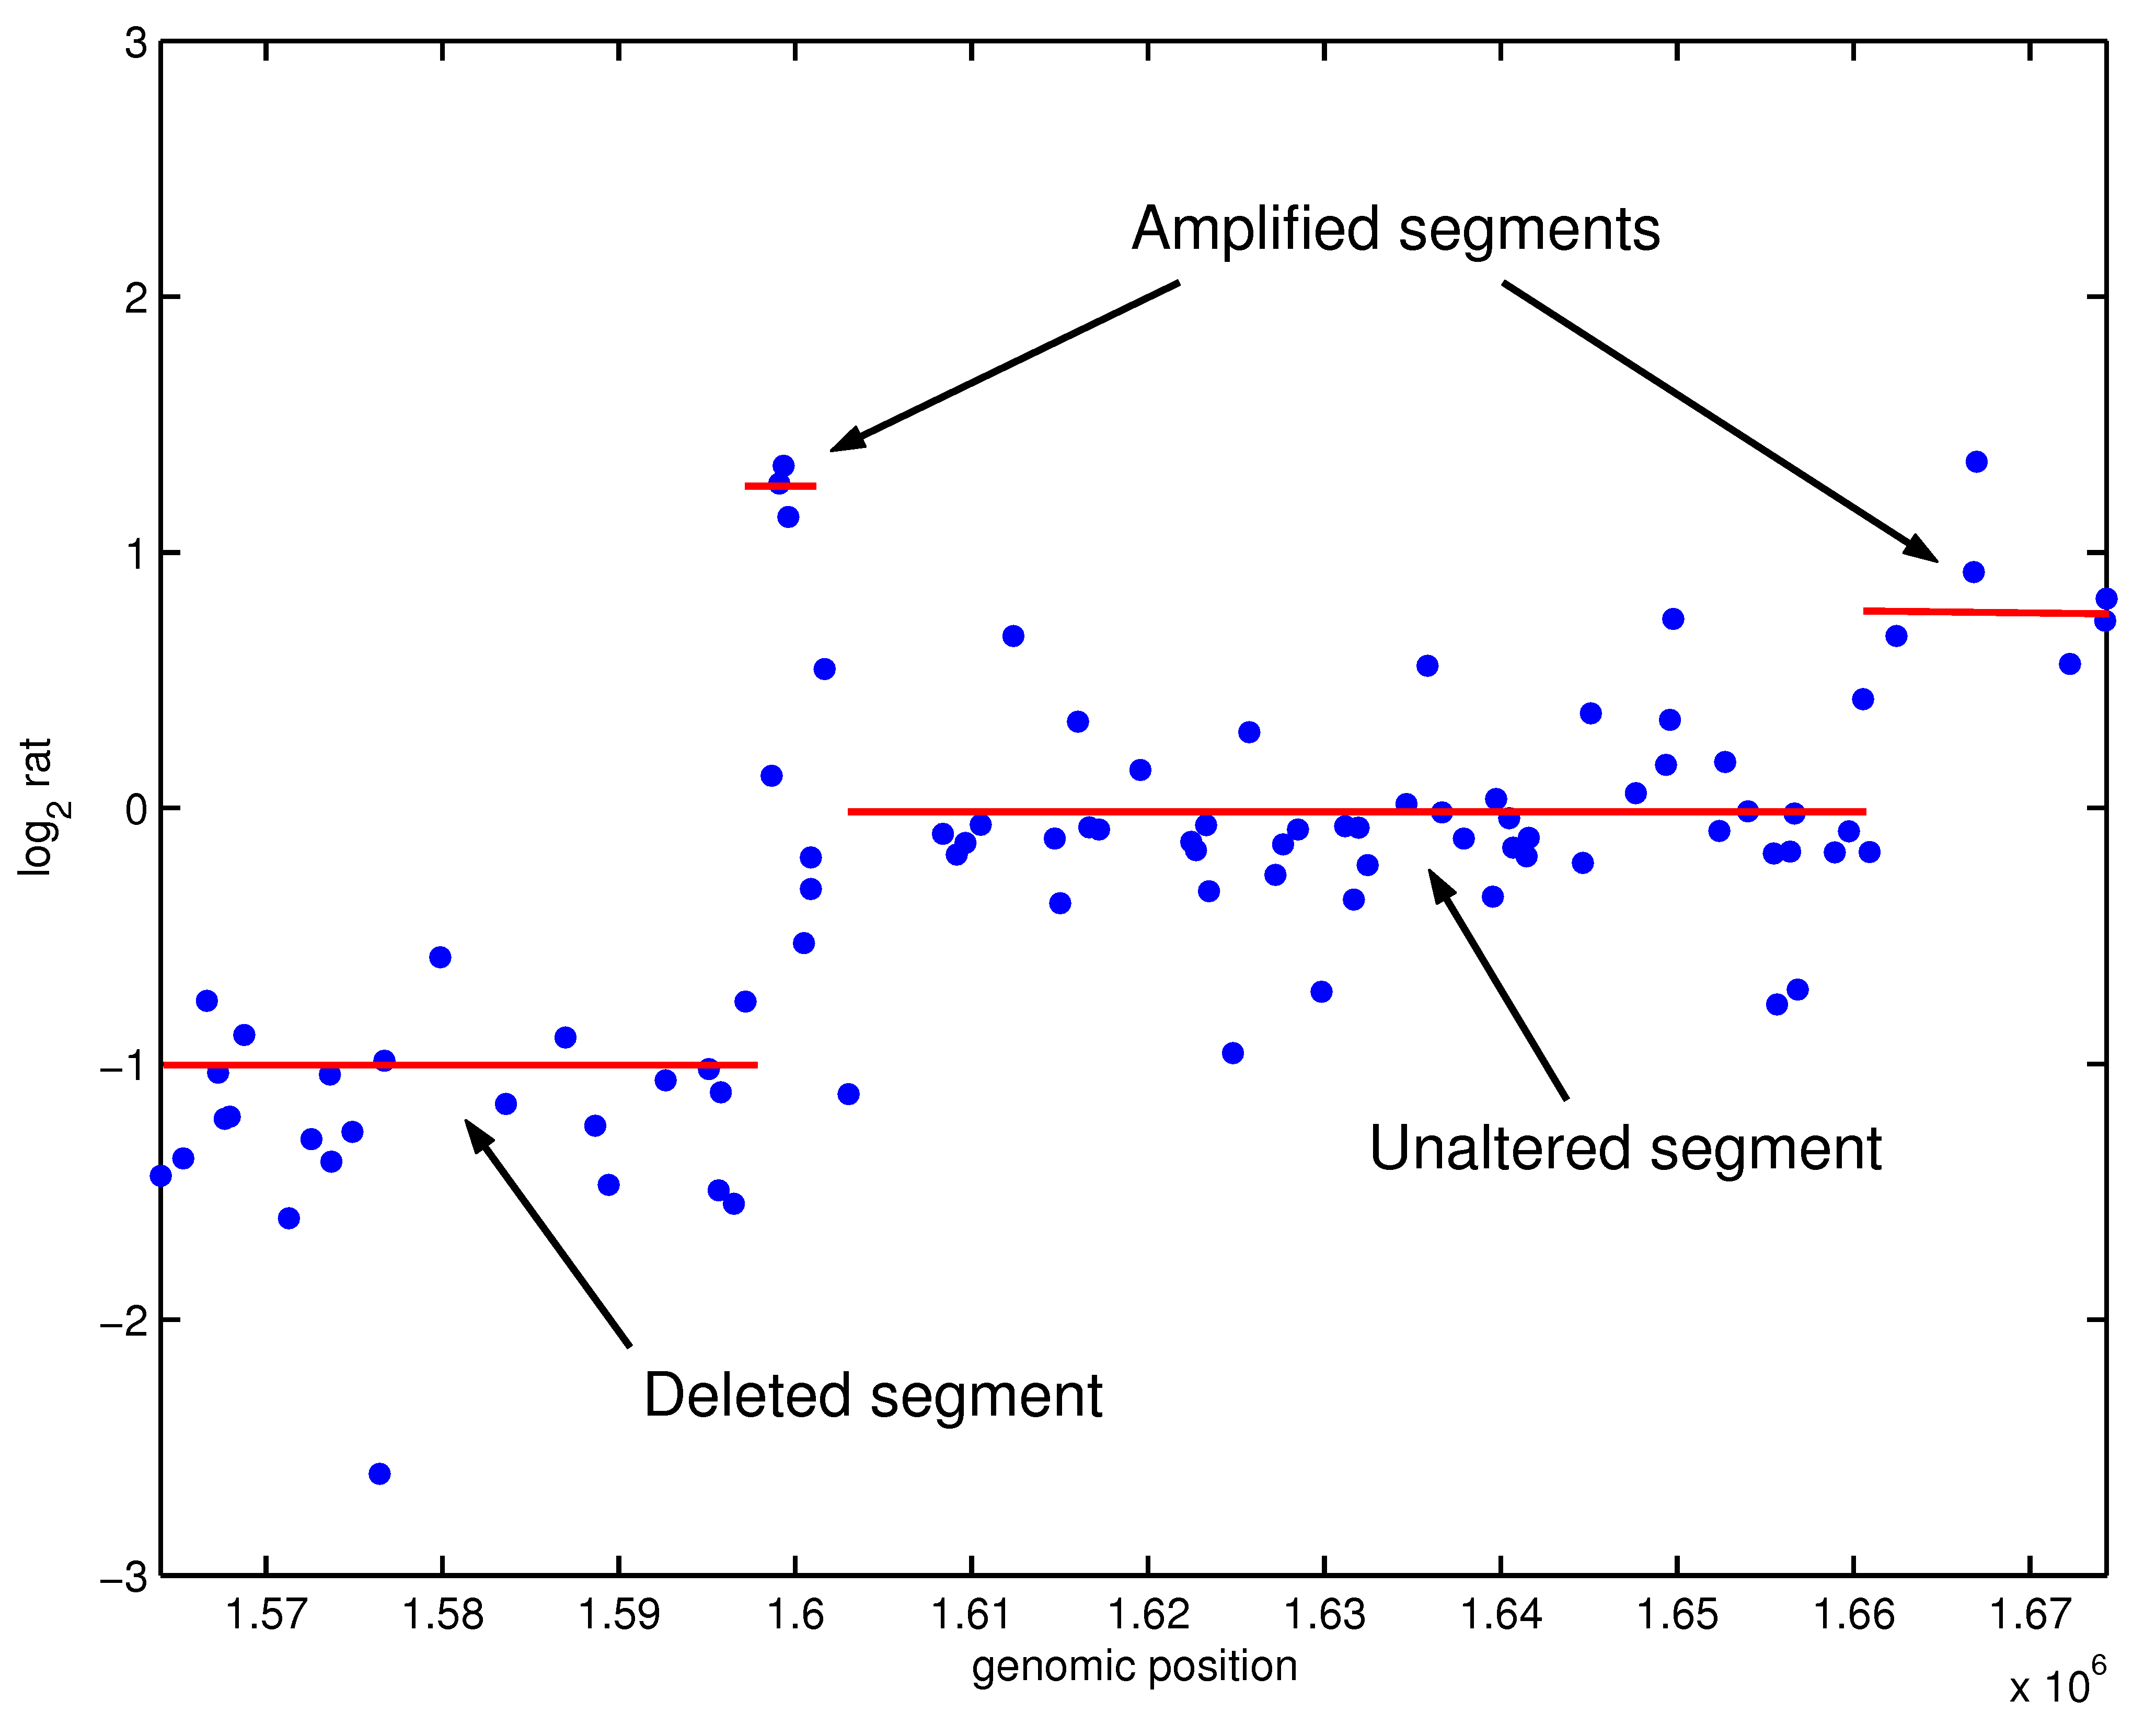
\epsfig{file = ../Figures/profile_example.eps, clip=,
  bbllx=60, bblly=196, bburx=543, bbury=586}
$$
\centerline{
  A dot on the graph 
  $
  \displaystyle{
    = \log_2 \left\{ \frac{\text{ $\sharp$ copies of BAC(t) in the test
          genome }}{\text{$\sharp$ copies of BAC(t) in the reference
          genome}}\right\}}
  $
}

%%%%%%%%%%%%%%%%%%%%%%%%%%%%%%%%%%%%%%%%%%%%%%%%%%%%%%%%%%
%%%%%%%%%%%%%%%%%%%%%%%%%%%%%%%%%%%%%%%%%%%%%%%%%%%%%%%%%%
\newpage
\chapter{A first modeling}
%%%%%%%%%%%%%%%%%%%%%%%%%%%%%%%%%%%%%%%%%%%%%%%%%%%%%%%%%%
%%%%%%%%%%%%%%%%%%%%%%%%%%%%%%%%%%%%%%%%%%%%%%%%%%%%%%%%%%

%%%%%%%%%%%%%%%%%%%%%%%%%%%%%%%%%%%%%%%%%%%%%%%%%%%%%%%%%%
\bigskip
\section{Break-points detection in a signal} 
\begin{itemize}
\item $Y_t =$ (random) log-ratio measured for the BAC number $t$.
\item The mean (and variance) of $Y_t$ changes at $(K-1)$ unknown
  coordinates $T=(t_1, ..., t_{K-1})$ ($\Rightarrow K$ segments).
\item The parameters of this model are: 
  \begin{eqnarray*}
    \mbox{the break point positions:} & T = & (t_1, ..., t_{K-1}), \\
    \\
    \mbox{the mean (and variance)} & & \\
    \mbox{of the log-ratio in each segment:} &
    \Theta = & (\mu_1, \sigma_1^2; \hdots; \mu_K,\sigma_K^2).
    \end{eqnarray*}
\end{itemize}
Break-points detection aims at studying the \textblue{spatial
    structure of the signal}.


%%%%%%%%%%%%%%%%%%%%%%%%%%%%%%%%%%%%%%%%%%%%%%%%%%%%%%%%%%
\newpage
%\subsection{Estimating the parameters in a model of abrupt-changes detection}
%%%%%%%%%%%%%%%%%%%%%%%%%%%%%%%%%%%%%%%%%%%%%%%%%%%%%%%%%%

\paragraph{Estimating the parameters with $K$ fixed by maximum likelihood}
\begin{itemize}
\item Joint estimation of $T$ and $\Theta$ with dynamic programming.
\item Dynamic programming works because the log-ratios are assumed to
  be independent (at least from one segment to another).
\end{itemize}

% \paragraph{Log-Likelihood} 
% $$
% \Lcal_K(T, \Theta)= \sum_{k=1}^K \log f(y^k;
% \theta_k)=\sum_{k=1}^K \sum_{t \in I_k}\log f(y_t; \theta_k)
% $$
\paragraph{Model Selection: choice of $K$}
\begin{itemize}
\item The fit of the modelling is measured by the likelihood of the
  data given the estimated parameters: $\Lcal_K$
\item Penalized Likelihood: 
  $$
  \hat{K} = \underset{K}{\arg\max}\left( \hat{\Lcal}_K - \beta K \right).
  $$
\item The parameter $\beta$ can be fixed, estimated or used as a
  tuning parameter.
\end{itemize}

%%%%%%%%%%%%%%%%%%%%%%%%%%%%%%%%%%%%%%%%%%%%%%%%%%%%%%%%%%
\newpage
\section{Example of segmentation on array CGH data}
%%%%%%%%%%%%%%%%%%%%%%%%%%%%%%%%%%%%%%%%%%%%%%%%%%%%%%%%%%

\paragraph{Are the variances $\sigma^2_k$ homogeneous?} BT474 cell
line, chromosome 9: 
$$
\begin{tabular}{cc}
  Homogeneous variances & Heterogeneous variances \\
  \multicolumn{2}{c}{$K=4$ segments} \\
  \epsfig{file = ../Figures/bt474_c9_seg_homo_K4.eps, clip=, scale=0.7} &
  \epsfig{file = ../Figures/bt474_c9_seg_hetero_K4.eps, clip=, scale=0.7} \\
\end{tabular}
$$

%%%%%%%%%%%%%%%%%%%%%%%%%%%%%%%%%%%%%%%%%%%%%%%%%%%%%%%%%%
\newpage
\paragraph{Adaptive choice of the number of segments.} BT474 cell
line, chromosome 1:
$$
\begin{tabular}{cc}
  Homogeneous variances & Heterogeneous variances \\
  $\widehat{K} = 10$  segments & $\widehat{K} = 2$ segments \\
  \epsfig{file = ../Figures/bt474_c1_seg_homo_K10.eps, clip=, scale=0.7} &
  \epsfig{file = ../Figures/bt474_c1_seg_hetero_K2.eps, clip=, scale=0.7} \\
\end{tabular}
$$
Homogeneous variances result in smaller segments.

%%%%%%%%%%%%%%%%%%%%%%%%%%%%%%%%%%%%%%%%%%%%%%%%%%%%%%%%%%
\newpage
\subsection{Comparative study} 

\paragraph{Lai \& al. (Bioinformatics, 05).} On both synthetic and
real data (GBM brain tumor data), the methods performs well.
$$
%\epsfig{file = ../Figures/LPJ05-Fig1.eps, clip=, scale=1.2}
%\epsfig{file = ../Figures/LPJ05-Fig3.eps, clip=, scale=1.2}
\epsfig{file = ../Figures/LPJ05-Fig4.eps, clip=, scale=1.2}
$$


%%%%%%%%%%%%%%%%%%%%%%%%%%%%%%%%%%%%%%%%%%%%%%%%%%%%%%%%%%
\newpage
\paragraph{ROC curves.} The sensitivity decreases for small segments
when  signal-to-noise ratio (SNR) is small.
$$
\epsfig{file = ../Figures/LPJ05-Fig2.eps, clip=, scale=1.2}
$$

%%%%%%%%%%%%%%%%%%%%%%%%%%%%%%%%%%%%%%%%%%%%%%%%%%%%%%%%%%
%%%%%%%%%%%%%%%%%%%%%%%%%%%%%%%%%%%%%%%%%%%%%%%%%%%%%%%%%%
\newpage
\chapter{A new model for segmentation-clustering}
%%%%%%%%%%%%%%%%%%%%%%%%%%%%%%%%%%%%%%%%%%%%%%%%%%%%%%%%%%
%%%%%%%%%%%%%%%%%%%%%%%%%%%%%%%%%%%%%%%%%%%%%%%%%%%%%%%%%%

\bigskip
\paragraph{Considering biologists objective and the need for a new
  model.}
$$
\begin{tabular}{cc}
  \epsfig{file = ../Figures/FigSegClas-1.eps, clip=, scale=0.7} &
  \epsfig{file = ../Figures/FigSegClas-2.eps, clip=, scale=0.7} \\
\end{tabular}
$$
We'd like segments of same type ('normal', 'deleted', amplified',
{\it etc.}) to be gathered into groups.
% $$
% \epsfig{file = ../Figures/nouveau_modele.ps, angle=270, clip=,
%   bbllx=92, bblly=47, bburx=484, bbury=828, scale=0.9}
% $$

%%%%%%%%%%%%%%%%%%%%%%%%%%%%%%%%%%%%%%%%%%%%%%%%%%%%%%%%%%
\newpage
\paragraph{Mixture Model of segments:} 
\begin{itemize}
\item We suppose there exists a \textblue{secondary underlying
    structure} of the segments into $P$ populations:
  $$
  \pi_p = \mbox{proportion of group $p$}
%   (Z_{k1},\hdots,Z_{kP}) \sim \mathcal{M}(1;\pi_1,\hdots,\pi_P).
  $$
\item Conditionally to the group to which the segment belongs, we know
  the distribution of $Y$:
  $$
  \mbox{BAC } t \mbox{ belongs to a segment of group } p \quad
  \Rightarrow \quad Y_t \mbox{ has mean } m_p \mbox{ (and variance } s_p^2).
%   Y^k|Z_{kp}=1 \sim \Ncal({\bf 1}_{n_k} m_p, s_p^2 {\bf I}_{n_k}).
  $$
%\item It is a model of \textblue{segmentation/clustering}.
\item The parameters of this model are
  \begin{eqnarray*}
    \mbox{the brakpoint positions:} \quad T&=&(t_1, ..., t_{K-1}),\\
    \mbox{the mixture characteristics:} \quad
    \Theta&=&(\pi_1,\hdots,\pi_P;m_1, \hdots, m_P; s_1^2, \hdots ,s_P^2).
  \end{eqnarray*}
\end{itemize}

% %%%%%%%%%%%%%%%%%%%%%%%%%%%%%%%%%%%%%%%%%%%%%%%%%%%%%%%%%%
% \newpage
% \section{Likelihood and statistical units of the model }
% %%%%%%%%%%%%%%%%%%%%%%%%%%%%%%%%%%%%%%%%%%%%%%%%%%%%%%%%%%


% \vspace{-0.5cm}    \mbox{the brakpoint positions:} \quad 
% \begin{itemize}
% \item the statistical units are segments:$Y^k$,
% \item the density of $Y^k$ is a mixture density:
%   $$
%   \log \Lcal_{KP}(T, \Theta)= \sum_{k=1}^K \log
%   f(y^k;\Theta)=\sum_{k=1}^K \log \left\{ \sum_{p=1}^P \pi_p
%     f(y^k;\theta_p) \right\}
%   $$
% \item \vspace{-0.5cm} If the $Y_ts$ are independent, we have:
%   $$
%   \log \Lcal_{KP}(T,\Theta) =\textcolor{red}{\sum_{k=1}^K} \log
%   \left\{ \textcolor{blue}{\sum_{p=1}^P} \pi_p \textcolor{red}{\prod_{
%         t \in I_k }}f(y_t; \theta_p) \right\}. 
%   $$
%   instead of $ \log \Lcal_{P}(\Theta) =
%   \textcolor{red}{\sum_{k=1}^K} \log \left\{ \textcolor{red}{\prod_{ t
%         \in I_k }} \textcolor{blue}{\sum_{p=1}^P} \pi_p f(y_t;
%     \theta_p)\right \} $ in the classical mixture model where the
%   statistical units are the elementary data $Y_t$s.
% \end{itemize}

%%%%%%%%%%%%%%%%%%%%%%%%%%%%%%%%%%%%%%%%%%%%%%%%%%%%%%%%%%
\newpage
\section{An hybrid estimation algorithm}
%%%%%%%%%%%%%%%%%%%%%%%%%%%%%%%%%%%%%%%%%%%%%%%%%%%%%%%%%%

\paragraph{Alternate parameters estimation with $K$ and $P$ known}
\begin{enumerate}
\item When $T$ is fixed, the \textblue{Expectation-Maximisation (EM)}
  algorithm estimates $\Theta$:
  $$
  T = (t_1, \dots, t_{K-1}) \quad \rightarrow \quad \Theta =
  (\pi_1,\hdots,\pi_P;m_1, \hdots, m_P; s_1^2, \hdots ,s_P^2)
  $$
\item When $\Theta$ is fixed, \textblue{dynamic programming} estimates $T$:
  $$
  \Theta = (\pi_1,\hdots,\pi_P;m_1, \hdots, m_P; s_1^2, \hdots
  ,s_P^2) \quad \rightarrow \quad T = (t_1, \dots, t_{K-1})
  $$
\end{enumerate} 

\paragraph{An increasing sequence  of likelihoods:}
At each step (1 or 2), the likelihood increases 
$$
\Rightarrow \mbox{ the algorithm converges}.
$$

% %%%%%%%%%%%%%%%%%%%%%%%%%%%%%%%%%%%%%%%%%%%%%%%%%%%%%%%%%%
% \newpage
% \subsection{Mixture Model when the segmentation is known}
% %%%%%%%%%%%%%%%%%%%%%%%%%%%%%%%%%%%%%%%%%%%%%%%%%%%%%%%%%%

% \paragraph{Mixture model parameters estimators.}
% \begin{eqnarray}
% \mbox{posterior probability:} \qquad \hat{\tau}_{kp} & = & \frac{\hat{\pi}_p f(y^k; \hat{\theta}_p)}{\suml \hat{\pi}_{\ell} f(y^k; \hat{\theta}_{\ell})}. \nonumber
% \end{eqnarray}
% \begin{itemize}
% \item the estimator the the mixing proportions is: $\hat{\pi}_p = \frac{\sumtau}{K}$.
% \item In the gaussian case, $\theta_p=(m_p,s_p^2)$: 
% \begin{eqnarray}
% \mbox{weighted mean:} \qquad \hat{m}_p   &=&  \frac{\sumtau \sumt y_t}{\sumtau n_k}, \nonumber \\
% \mbox{weighted variance:} \qquad \hat{s}_p^2 &=&  \frac{\sumtau \sumt (y_t- \hat{m}_p)^2}{\sumtau n_k}. \nonumber 
% \end{eqnarray}
% \item Big size vectors will have a bigger impact in the estimation of the parameters, via the term $\sumtau n_k$ \\
% \end{itemize}

% %%%%%%%%%%%%%%%%%%%%%%%%%%%%%%%%%%%%%%%%%%%%%%%%%%%%%%%%%%
% \newpage
% \subsection{Segmentation with a fixed mixture}
% %%%%%%%%%%%%%%%%%%%%%%%%%%%%%%%%%%%%%%%%%%%%%%%%%%%%%%%%%%

% \paragraph{Back to dynamic programming}
% \begin{itemize}
% \item the incomplete mixture log-likelihood can be written as a sum of local log-likelihoods:
%   $$
%   \begin{array}{ccccc}
%     \Lcal_{KP}(T,\Theta) & = & \sumk \ell_{kP}(y^k;\Theta) 
%   \end{array}
%   $$
% \item the local log-likelihood of segment $k$ corresponds to the
%   mixture log-density of vector $Y^k$
%   $$
%   \ell_{kP}(y^k;\Theta)=\log \left\{\sum_{p=1}^P \pi_p \prod_{t \in
%       I_k} f(y_t;\theta_p)\right\}.
%   $$
% \item $\log \Lcal_{KP}(T,\Theta)$ can be optimized in $T$ with $\Theta$ fixed, by dynamix programming. 
% \end{itemize}

%%%%%%%%%%%%%%%%%%%%%%%%%%%%%%%%%%%%%%%%%%%%%%%%%%%%%%%%%%%
\newpage
\section{Model selection: $K=?$, $P=?$}
%%%%%%%%%%%%%%%%%%%%%%%%%%%%%%%%%%%%%%%%%%%%%%%%%%%%%%%%%%%

\subsection{Choosing the number of groups $P$} 

\vspace{-0.5cm}
We use the BIC criterion:
$$
BIC = \Lcal_{P} - \log n \times (\# \mbox{ of parameters}) / 2
$$
\vspace{-1cm}
$$
\begin{tabular}{cc}
  Simulated sequence & $\Lcal_{KP}$ and $BIC$ criterion \\
  \epsfig{file = ../Figures/Exemple_P2K4.eps, clip=, scale=0.7} &
  \epsfig{file = ../Figures/Exemple_P2K4_BIC.eps, clip=, scale=0.7} \\
\end{tabular}
$$
The log-likelihood $\Lcal$ (\textred{\bf ---}) always increases with
$P$ while $BIC$ ({\bf ---}) has a maximum.

%%%%%%%%%%%%%%%%%%%%%%%%%%%%%%%%%%%%%%%%%%%%%%%%%%%%%%%%%%%
\newpage
\subsection{Choosing the number of segments $K$} 

The likelihood may decrease when $K$ increases:
$$
\begin{tabular}{lc}
  \hspace{-1cm}
  \begin{tabular}{l}
    Simulated data: \\
    \\
    $f(y^k;\Theta) =$ \\
    \\
    $0.5 \Ncal(0,1)+ 0.5 \Ncal(5,1)$ \\
    \\
    \\
    Log-likelihood $\Lcal_{KP}$ \\
    as a function of $K$ \\
    \\
    ($P=2$) \\
    \\
  \end{tabular}
  & \begin{tabular}{c}
    \epsfig{file = ../Figures/simulation_2.eps, clip=, scale=0.8}
  \end{tabular}
\end{tabular}
$$
$\rightarrow$ sort of self-penalization of the log-likelihood with
respect to $K$.

%%%%%%%%%%%%%%%%%%%%%%%%%%%%%%%%%%%%%%%%%%%%%%%%%%%%%%%%%%%
\newpage
\section{Example: CGH for BT474 cell line}
%%%%%%%%%%%%%%%%%%%%%%%%%%%%%%%%%%%%%%%%%%%%%%%%%%%%%%%%%%%

\paragraph{Interest of clustering: an easy case.} Chromosome 9:
$$
  \begin{tabular}{cc}
    Segmentation & Segmentation/Clustering \\
    \multicolumn{2}{c}{$K=4$ segments} \\
    \epsfig{file = ../Figures/bt474_c9_seg_homo_K4, clip=, scale=0.7} 
    & 
    \epsfig{file = ../Figures/bt474_c9_segclas_homo_P3K4 , clip=, scale=0.7} 
  \end{tabular}
$$
Clustering defines 'deleted', 'normal' and 'amplified' groups.

\newpage

\paragraph{Interest of clustering: a more interesting case.}
Chromosome 1:
$$
\begin{tabular}{cc}
  Segmentation & Segmentation/Clustering \\
  $K=2$ & $P=3$, $K=8$ \\
  \epsfig{file = ../Figures/bt474_c1_seg_hetero_K2.eps, clip=, scale=0.7} 
  & \epsfig{file = ../Figures/resultat_P3K8.eps , clip=, scale=0.7} 
\end{tabular}
$$
Clustering detects an outliers and captures a 'normal' segment within
a large variance region.


%%%%%%%%%%%%%%%%%%%%%%%%%%%%%%%%%%%%%%%%%%%%%%%%%%%%%%%%%%%
%%%%%%%%%%%%%%%%%%%%%%%%%%%%%%%%%%%%%%%%%%%%%%%%%%%%%%%%%%%
\newpage
\chapter{Conclusion and future works}
%%%%%%%%%%%%%%%%%%%%%%%%%%%%%%%%%%%%%%%%%%%%%%%%%%%%%%%%%%%
%%%%%%%%%%%%%%%%%%%%%%%%%%%%%%%%%%%%%%%%%%%%%%%%%%%%%%%%%%%

\paragraph{What we did:}
\vspace{-0.5cm}
\begin{itemize}
\item Definition of a new model that considers the \textit{a priori}
  knowledge we have about the biological phenomena under study.
\item Development of an hybrid algorithm (EM/dynamic programming) for
  the parameters estimation (problems linked to EM: initializtion,
  local maxima, degeneracy).
\item Still waiting for an other data set to assess the performance of
  the clustering.
\end{itemize}

\paragraph{What we still have to do:}
\vspace{-0.5cm}
\begin{itemize}
\item Modeling: Comparison with Hidden Markov Models
\item Model choice: Develop an adaptive procedure for two components.
\item Other application field: DNA sequences (in progress)
\end{itemize}


%%%%%%%%%%%%%%%%%%%%%%%%%%%%%%%%%%%%%%%%%%%%%%%%%%%%%%%%%%%%%%%%%%%%%%
%%%%%%%%%%%%%%%%%%%%%%%%%%%%%%%%%%%%%%%%%%%%%%%%%%%%%%%%%%%%%%%%%%%%%%
%%%%%%%%%%%%%%%%%%%%%%%%%%%%%%%%%%%%%%%%%%%%%%%%%%%%%%%%%%%%%%%%%%%%%%
%%%%%%%%%%%%%%%%%%%%%%%%%%%%%%%%%%%%%%%%%%%%%%%%%%%%%%%%%%%%%%%%%%%%%%
\end{document}
%%%%%%%%%%%%%%%%%%%%%%%%%%%%%%%%%%%%%%%%%%%%%%%%%%%%%%%%%%%%%%%%%%%%%%
%%%%%%%%%%%%%%%%%%%%%%%%%%%%%%%%%%%%%%%%%%%%%%%%%%%%%%%%%%%%%%%%%%%%%%
%%%%%%%%%%%%%%%%%%%%%%%%%%%%%%%%%%%%%%%%%%%%%%%%%%%%%%%%%%%%%%%%%%%%%%
%%%%%%%%%%%%%%%%%%%%%%%%%%%%%%%%%%%%%%%%%%%%%%%%%%%%%%%%%%%%%%%%%%%%%%
